\begin{figure}[H]
    \centering
    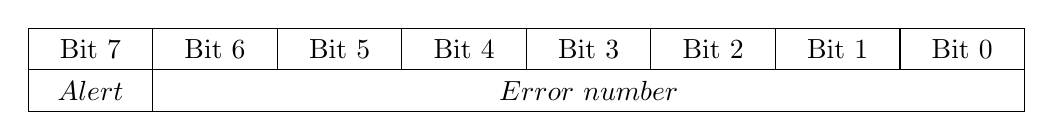
\begin{tikzpicture}[x=0.75pt,y=0.75pt,yscale=-1,xscale=1]
%uncomment if require: \path (0,158.99999237060547); %set diagram left start at 0, and has height of 158.99999237060547

%Shape: Rectangle [id:dp09142087079107619] 
\draw   (10,10) -- (70,10) -- (70,30) -- (10,30) -- cycle ;
%Shape: Rectangle [id:dp4629750443029259] 
\draw   (70,10) -- (130,10) -- (130,30) -- (70,30) -- cycle ;
%Shape: Rectangle [id:dp16194932941841267] 
\draw   (130,10) -- (190,10) -- (190,30) -- (130,30) -- cycle ;
%Shape: Rectangle [id:dp25658747620974176] 
\draw   (190,10) -- (250,10) -- (250,30) -- (190,30) -- cycle ;
%Shape: Rectangle [id:dp4454573381940983] 
\draw   (250,10) -- (310,10) -- (310,30) -- (250,30) -- cycle ;
%Shape: Rectangle [id:dp2107426327299584] 
\draw   (310,10) -- (370,10) -- (370,30) -- (310,30) -- cycle ;
%Shape: Rectangle [id:dp742699471984243] 
\draw   (370,10) -- (430,10) -- (430,30) -- (370,30) -- cycle ;
%Shape: Rectangle [id:dp768648200139064] 
\draw   (430,10) -- (490,10) -- (490,30) -- (430,30) -- cycle ;
%Shape: Rectangle [id:dp3416120520607919] 
\draw   (10,30) -- (70,30) -- (70,50) -- (10,50) -- cycle ;
%Shape: Rectangle [id:dp9451706315688295] 
\draw   (70,30) -- (490,30) -- (490,50) -- (70,50) -- cycle ;

% Text Node
\draw (40,20) node  [align=left] {Bit 7};
% Text Node
\draw (100,20) node  [align=left] {Bit 6};
% Text Node
\draw (160,20) node  [align=left] {Bit 5};
% Text Node
\draw (220,20) node  [align=left] {Bit 4};
% Text Node
\draw (280,20) node  [align=left] {Bit 3};
% Text Node
\draw (340,20) node  [align=left] {Bit 2};
% Text Node
\draw (400,20) node  [align=left] {Bit 1};
% Text Node
\draw (460,20) node  [align=left] {Bit 0};
% Text Node
\draw (40,40) node   {$Alert$};
% Text Node
\draw (280,40) node   {$Error\ number$};


\end{tikzpicture}

    \caption{Error structure\cite{PIDmxx}}
    \label{fig:Errorstruct}
\end{figure}